% =====================================================================
%  Substitution-Tolerant Structural Correspondence
%
%  Self-contained.  Every construction is defined here.
% =====================================================================
\documentclass[11pt,a4paper]{article}

\usepackage[utf8]{inputenc}
\usepackage[T1]{fontenc}
\usepackage{lmodern}
\usepackage[a4paper,margin=2.4cm]{geometry}
\usepackage{amsmath,amssymb,amsthm,mathtools}
\usepackage{bm}
\usepackage{booktabs}
\usepackage{array}
\usepackage{longtable}
\usepackage{enumitem}
\usepackage{microtype}
\usepackage{xcolor}
\usepackage{graphicx}
\graphicspath{{figures/}}
\usepackage[round,sort&compress]{natbib}
\usepackage[colorlinks=true,linkcolor=blue!45!black,
            citecolor=blue!45!black,urlcolor=blue!45!black]{hyperref}
\usepackage{cleveref}

\newtheoremstyle{scthm}{\topsep}{\topsep}{\itshape}{}{\bfseries}{.}{.5em}{}
\theoremstyle{scthm}
\newtheorem{theorem}{Theorem}[section]
\newtheorem{lemma}[theorem]{Lemma}
\newtheorem{proposition}[theorem]{Proposition}
\newtheorem{corollary}[theorem]{Corollary}
\theoremstyle{definition}
\newtheorem{definition}[theorem]{Definition}
\newtheorem{example}[theorem]{Example}
\theoremstyle{remark}
\newtheorem{remark}[theorem]{Remark}

\newcommand{\R}{\mathbb{R}}
\newcommand{\N}{\mathbb{N}}
\newcommand{\Gph}{\Gamma}
\newcommand{\V}{V}
\newcommand{\E}{E}
\newcommand{\wt}{w}
\newcommand{\med}{\mathsf{m}}
\newcommand{\cut}{\partial}
\newcommand{\sep}{\sigma}
\newcommand{\dep}{d}
\newcommand{\key}{\kappa}
\newcommand{\lab}{\lambda}
\newcommand{\abs}[1]{\lvert#1\rvert}
\newcommand{\Aut}{\operatorname{Aut}}

\title{\textbf{Substitution-Tolerant Structural Correspondence}\\[6pt]
\large Matching Molecules on Cut Classes Rather Than on Element
Identity,\\ with Tolerance as an Explicit Resolution Parameter}

\author{%
Kundai Farai Sachikonye\\
\small Technical University of Munich\\
\small \texttt{kundai.sachikonye@wzw.tum.de}}

\date{\today}

\begin{document}
\maketitle

\begin{abstract}
\noindent
Structural matching in cheminformatics---substructure search, maximum
common substructure, scaffold comparison---is keyed on atom identity: a
carbon may correspond only to a carbon. This is the right constraint when
the question is whether one structure contains another, and the wrong one
when the question is whether two structures play the same structural role,
because a heteroatom substitution that a medicinal chemist regards as
conservative is, to an element-keyed matcher, a complete mismatch at that
position.

We define a correspondence keyed on a graph invariant instead. Each atom
is labelled by its \emph{cut key}: the minimum weight of a cut separating
it from a distinguished medium vertex, together with the number of atoms
on the minimising side. Two atoms may correspond when their cut keys
agree, which permits a carbon and a nitrogen in equivalent structural
positions to pair while forbidding a ring carbon and a chain carbon from
doing so. We prove the correspondence is symmetric, invariant under
relabelling, and computable without search (\Cref{thm:symmetry},
\Cref{thm:invariance}, \Cref{prop:cost}), in contrast to maximum common
substructure, which is $\mathsf{NP}$-hard.

The paper's main structural claim is that \emph{tolerance is a resolution
parameter}, not a threshold on a score. Iterating the cut key under
neighbour refinement produces a family of labellings indexed by radius;
higher radius discriminates more and therefore tolerates less. We
predicted that the coarsest radius would separate bioisosteric pairs from
unrelated pairs best, and measured a radius sweep to check it. The
prediction held: at radius $0$ the separation margin between bioisosteric
and unrelated pairs is $+0.375$, and at radii $1$, $2$ and $3$ it is
exactly $0$ in each case. This inverts the intuition that a better
matcher should discriminate more.

At the working radius the mean class overlap is $0.780$ for bioisosteric
pairs against $0.050$ for unrelated pairs of comparable size, with
disjoint ranges. Correspondence coverage on eight matched pairs differing
at one position averages $0.776$. A negative control that rewires a
structure at random, holding atom composition and edge count fixed,
collapses the margin from $+0.375$ to $-0.069$.

We report two experiment-design errors found during the work, because both
changed a conclusion: an element baseline that was not a baseline, and a
negative control that could not fail. We also report a result that is
weaker than we expected---the cross-element pairings the method admits and
an element-keyed matcher cannot number only $4$ across six bioisosteric
pairs---and we state plainly that this is the paper's least convincing
measurement.
\end{abstract}

\noindent\textbf{Keywords:} structural correspondence; maximum common
substructure; bioisosterism; graph invariant; minimum cut; molecular
similarity; scaffold hopping.

\tableofcontents

% =====================================================================
\section{Introduction}
\label{sec:intro}
% =====================================================================

\subsection{Two questions that need different matchers}

``Does molecule $A$ contain molecule $B$?'' and ``do molecules $A$ and $B$
play the same structural role?'' are different questions, and the second
is not a relaxation of the first.

The first is subgraph isomorphism, solved by well-understood algorithms
\citep{ullmann1976,cordella2004,ehrlich2012}. Its correctness condition
requires atom identity to be respected: a match that paired a carbon with
a nitrogen would not be a substructure match at all. The second question
underlies scaffold hopping \citep{schneider1999,brown2006}, bioisostere
replacement \citep{patani1996,meanwell2011,wirth2013}, and matched-pair
analysis \citep{griffen2011,hussain2010}, and for these the element
constraint is precisely what gets in the way: replacing a benzene by a
pyridine is a canonical conservative substitution, and an element-keyed
matcher scores that position as a total mismatch.

The usual response is to soften the score rather than the matcher---to
compute a fingerprint similarity \citep{rogers2010,willett1998,maggiora2014}
and accept that similar molecules score highly. That works, but it
produces a number rather than a correspondence: it does not say which atom
of $A$ plays the role of which atom of $B$, which is what a medicinal
chemist reading a matched pair actually wants.

\subsection{What we propose}

Label each atom by a graph invariant that is indifferent to element, and
match on the label.

The invariant is a minimum cut. Fix a weighted graph on the atoms with an
additional \emph{medium} vertex adjacent to every atom. For an atom $v$
let $\sep(v)$ be the minimum weight of a cut separating $v$ from the
medium and $\dep(v)$ the number of atoms on the minimising side; the
\emph{cut key} is $\key(v)=(\sep(v),\dep(v))$. Two atoms may correspond
when their cut keys agree.

This is tolerant in the right direction. A nitrogen replacing a carbon in
an aromatic ring occupies the same structural position and receives a
comparable cut key, so the atoms may correspond. A carbon in a ring and a
carbon in a side chain occupy different positions and receive different
keys, so they may not---even though an element-keyed matcher would
happily pair them.

\subsection{Tolerance is a resolution parameter}

The cut key can be refined: replace each label by the pair of itself and
the multiset of its neighbours' labels, and iterate. Each round
discriminates more.

That gives a family of matchers indexed by refinement radius, and it makes
the paper's central design question sharp. A matcher's tolerance is
inversely related to its discrimination, so \emph{the coarsest radius
should tolerate most}. We stated this as a prediction before measuring and
report the sweep in \Cref{sec:validation}: the coarsest radius separates
bioisosteric from unrelated pairs with a margin of $+0.375$, and every
finer radius gives exactly $0$.

We emphasise this because it runs against the natural instinct, which is
that a matcher should be made more discriminating to be made better. For
this task it should be made less.

\subsection{What we claim and what we do not}

We claim: the correspondence is symmetric, invariant, and computable
without search; tolerance behaves as a resolution parameter with the
coarsest radius best; and on a small hand-assembled corpus the class
overlap separates bioisosteric from unrelated pairs with disjoint ranges,
a separation a rewiring control destroys.

We do not claim: that the correspondence is a maximum common substructure
(it is not, and \Cref{sec:limits} says why); that it is a similarity
measure validated against activity data (we have not measured any); that
the corpus is representative; or that the cross-element gain is large---it
is $4$ pairings across six molecule pairs, which is the weakest number in
the paper and is reported as such.

% =====================================================================
\section{Setting}
\label{sec:setting}
% =====================================================================

\begin{definition}[Contact graph]
\label{def:graph}
A \emph{contact graph} is $\Gph=(\V,\E,\wt,\med)$ with $\V$ finite and
non-empty, $\E\subseteq\binom{\V}{2}$, $\wt\colon\E\to\R_{>0}$, and a
distinguished vertex $\med$ adjacent to every other. Vertices other than
$\med$ are \emph{items}, written $I=\V\setminus\{\med\}$; $N(v)$ denotes
the item neighbours of $v$.
\end{definition}

\begin{definition}[Cut key]
\label{def:key}
For $S\subseteq\V$ let $\cut(S)$ be its edge boundary and
$\wt(\cut(S))$ the sum of the weights therein. For an item $v$,
\[
\sep(v)=\min_{S\ni v,\ \med\notin S}\wt(\cut(S)),
\qquad
\dep(v)=\min\{\abs{S\cap I}: S\text{ attains the minimum}\},
\]
and the \emph{cut key} is $\key(v)=(\sep(v),\dep(v))$.
\end{definition}

The minimum is attained on a finite family and equals a maximum flow
\citep{fordfulkerson1956}, computable in polynomial time
\citep{stoer1997}. Since $\{v,\med\}\in\E$, every admissible cut is
non-empty, so $\sep(v)>0$ and $\dep(v)\ge1$.

\begin{definition}[Labels at radius $r$]
\label{def:radius}
Set $\lab_0(v)=\key(v)$, and for $r\ge1$
\begin{equation}
\lab_r(v)=\bigl(\lab_{r-1}(v),\
\langle\!\langle \lab_{r-1}(u):u\in N(v)\rangle\!\rangle\bigr),
\label{eq:refine}
\end{equation}
with $\langle\!\langle\cdot\rangle\!\rangle$ a multiset in canonical
order. Write $C_r(\Gph)$ for the multiset
$\langle\!\langle \lab_r(v):v\in I\rangle\!\rangle$.
\end{definition}

\begin{lemma}[Radius is a discrimination order]
\label{lem:radius-order}
For every $r$, the partition of $I$ induced by $\lab_{r+1}$ refines that
induced by $\lab_r$. Consequently the number of distinct labels is
non-decreasing in $r$, and two atoms that differ at radius $r$ differ at
every radius $r'>r$.
\end{lemma}

\begin{proof}
If $\lab_{r+1}(u)=\lab_{r+1}(v)$ then their first components agree, so
$\lab_r(u)=\lab_r(v)$. That is the refinement relation; the cardinality
and persistence claims follow immediately.
\end{proof}

\Cref{lem:radius-order} is what makes ``tolerance is a resolution
parameter'' precise: a matcher keyed on $\lab_r$ identifies strictly fewer
pairs of atoms as it grows $r$, so tolerance is monotonically decreasing
in radius.

% =====================================================================
\section{Correspondence}
\label{sec:correspondence}
% =====================================================================

\begin{definition}[Class-respecting correspondence]
\label{def:corr}
Let $\Gph_1,\Gph_2$ be contact graphs and fix a radius $r$. For each
label $\ell$ let $A_\ell$ and $B_\ell$ be the items of $\Gph_1$ and
$\Gph_2$ carrying it. The \emph{correspondence at radius $r$} is
\[
M_r(\Gph_1,\Gph_2)=\bigcup_{\ell}\ \bigl\{(a_i,b_i): 1\le i\le
\min(\abs{A_\ell},\abs{B_\ell})\bigr\},
\]
where $a_i$ and $b_i$ enumerate $A_\ell$ and $B_\ell$ in a fixed order.
Its \emph{size} is $\abs{M_r}$ and its \emph{coverage} is
$\abs{M_r}/\max(\abs{I_1},\abs{I_2})$.
\end{definition}

\begin{theorem}[Symmetry]
\label{thm:symmetry}
$\abs{M_r(\Gph_1,\Gph_2)}=\abs{M_r(\Gph_2,\Gph_1)}$ for every $r$.
\end{theorem}

\begin{proof}
The size is $\sum_\ell \min(\abs{A_\ell},\abs{B_\ell})$, and $\min$ is
symmetric in its arguments. Exchanging the graphs exchanges $A_\ell$ with
$B_\ell$ for every $\ell$ and leaves each summand unchanged.
\end{proof}

\begin{theorem}[Invariance]
\label{thm:invariance}
If $\phi_1\colon\Gph_1\to\Gph_1'$ and $\phi_2\colon\Gph_2\to\Gph_2'$ are
weighted isomorphisms fixing the medium, then
$\abs{M_r(\Gph_1',\Gph_2')}=\abs{M_r(\Gph_1,\Gph_2)}$ for every $r$.
\end{theorem}

\begin{proof}
A weighted isomorphism carries admissible cuts to admissible cuts of equal
weight and restricts to a bijection on items, so $\sep$ and $\dep$---and
hence $\key$---are preserved; this is the base case. It also restricts to
a bijection on item neighbourhoods, so by induction on $r$ using
\eqref{eq:refine}, $\lab_r$ is preserved. Therefore the label classes
correspond under $\phi_1,\phi_2$ with equal sizes, and the sum
$\sum_\ell\min(\abs{A_\ell},\abs{B_\ell})$ is unchanged.
\end{proof}

\begin{proposition}[No search]
\label{prop:cost}
With $n=\max(\abs{I_1},\abs{I_2})$, $m$ the edge count, and $F(n,m)$ the
cost of one maximum flow, $M_r$ is computable in
$O(nF(n,m)+rm\log n+n\log n)$ time. In particular the cost is polynomial
and involves no backtracking.
\end{proposition}

\begin{proof}
One flow per item gives all cut keys; each refinement round sorts each
vertex's neighbour labels, $O(m\log n)$; grouping items by label and
zipping the groups is $O(n\log n)$.
\end{proof}

\Cref{prop:cost} is the sharpest contrast with maximum common
substructure, which is $\mathsf{NP}$-hard
\citep{garey1979,raymond2002,ehrlich2011} and is normally attacked by
clique detection on a modular product graph
\citep{barrow1976,bron1973,raymond2002rascal}. The present construction is
not solving that problem---see \Cref{sec:limits}---and its tractability is
a consequence of solving a weaker one.

\begin{definition}[Class overlap]
\label{def:overlap}
The \emph{class overlap} at radius $r$ is the Jaccard index of the label
multisets,
\[
J_r(\Gph_1,\Gph_2)=
\frac{\abs{C_r(\Gph_1)\cap C_r(\Gph_2)}}
     {\abs{C_r(\Gph_1)\cup C_r(\Gph_2)}},
\]
with multiset intersection and union.
\end{definition}

\begin{proposition}[Overlap is monotone in discrimination]
\label{prop:overlap-monotone}
If two atoms carry the same label at radius $r+1$ they carry the same
label at radius $r$. Hence every label class at radius $r+1$ is contained
in one at radius $r$, and $J_{r+1}\le J_r$ whenever the two structures'
label sets are related by that containment.
\end{proposition}

\begin{proof}
The containment is \Cref{lem:radius-order}. Splitting a shared class into
parts can only reduce or preserve the matched count in the numerator while
leaving the union no smaller, so the ratio does not increase.
\end{proof}

\Cref{prop:overlap-monotone} predicts the direction of the radius sweep
measured in \Cref{sec:validation}; the measurement is what determines the
magnitude and whether any radius other than $0$ retains discriminating
power.

% =====================================================================
\section{Validation}
\label{sec:validation}
% =====================================================================

\subsection{Method}

Expectations were written into the experiment source before the
experiment ran, and each is reported below with its measured outcome.
Every number is read from the emitted results file. Structures are parsed
from line notations \citep{weininger1988} into contact graphs; all minimum
cuts are exact. Counts are heavy-atom counts.

Three sets are used. \emph{Isostere pairs}: ten pairs, six annotated
\textsf{close} (widely treated as interchangeable in medicinal chemistry
\citep{patani1996,meanwell2011}) and four annotated \textsf{far} (similar
size, different structural class). The annotations were fixed before
measurement. \emph{Matched pairs}: eight pairs differing at one position.
\emph{Drug-like set}: thirty structures, used only descriptively.


\begin{figure*}[!htbp]
\centering
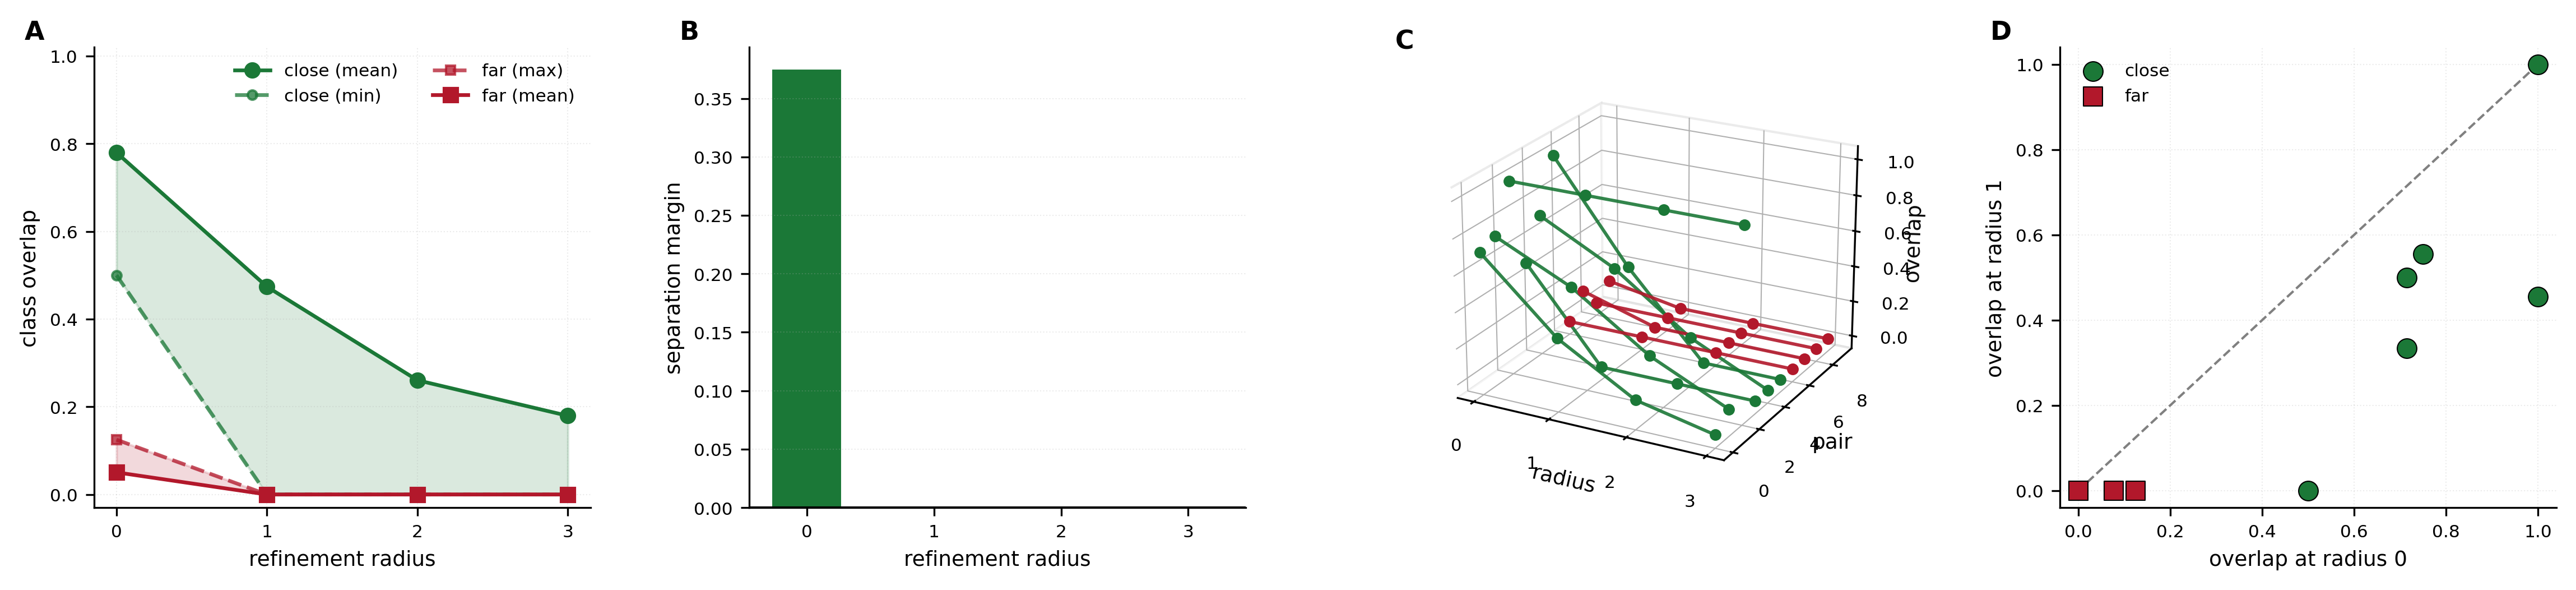
\includegraphics[width=\textwidth]{panel_01_radius.png}
\caption{\textbf{Tolerance is a resolution parameter: the coarsest radius
separates best.} (\textbf{A})~Mean class overlap against refinement radius for
the \textsf{close} (green) and \textsf{far} (red) groups, with the shaded bands
running to the minimum \textsf{close} and maximum \textsf{far} value; the bands
are disjoint only at radius $0$. (\textbf{B})~The separation margin, minimum
\textsf{close} minus maximum \textsf{far}, by radius: $+0.375$ at radius $0$ and
exactly $0$ at radii $1$, $2$ and $3$. (\textbf{C})~Every annotated pair traced
across all four radii in three dimensions, \textsf{close} in green and
\textsf{far} in red; the \textsf{close} traces descend toward the \textsf{far}
floor as radius grows. (\textbf{D})~Overlap at radius $1$ against overlap at
radius $0$ for each pair, with the identity line; every \textsf{close} pair falls
below the diagonal, and one falls to zero.}
\label{fig:radius}
\end{figure*}

\subsection{The radius sweep}

\begin{table}[htbp]
\centering\small
\caption{Class overlap by refinement radius. ``Margin'' is the minimum
overlap among \textsf{close} pairs minus the maximum among \textsf{far}
pairs; positive means the two groups do not overlap.}
\label{tab:sweep}
\begin{tabular}{@{}rrrrrr@{}}
\toprule
Radius & mean close & mean far & min close & max far & margin\\
\midrule
$0$ & $0.780$ & $0.050$ & $0.500$ & $0.125$ & $+0.375$\\
$1$ & $0.474$ & $0.000$ & $0.000$ & $0.000$ & $\phantom{+}0.000$\\
$2$ & $0.261$ & $0.000$ & $0.000$ & $0.000$ & $\phantom{+}0.000$\\
$3$ & $0.179$ & $0.000$ & $0.000$ & $0.000$ & $\phantom{+}0.000$\\
\bottomrule
\end{tabular}
\end{table}

The prediction was that radius $0$ would separate best.
\Cref{tab:sweep} confirms it, and the mechanism is visible: mean overlap
among \textsf{close} pairs falls monotonically with radius, exactly as
\Cref{prop:overlap-monotone} requires, and by radius $1$ it has fallen far
enough that the minimum reaches $0$ and the groups touch. Radius $0$ is
therefore the working radius for all subsequent measurements.

\begin{remark}[Why finer is worse here]
\label{rem:finer-worse}
At radius $1$ a label already encodes an atom's whole first
neighbourhood, so a nitrogen-for-carbon substitution changes not only that
atom's label but every neighbour's. One substitution perturbs a
neighbourhood's worth of labels, and the overlap collapses. This is
correct behaviour for a discriminating matcher and wrong behaviour for a
tolerant one, which is the point of \Cref{lem:radius-order}: the two are
the same dial turned opposite ways.
\end{remark}


\begin{figure*}[!htbp]
\centering
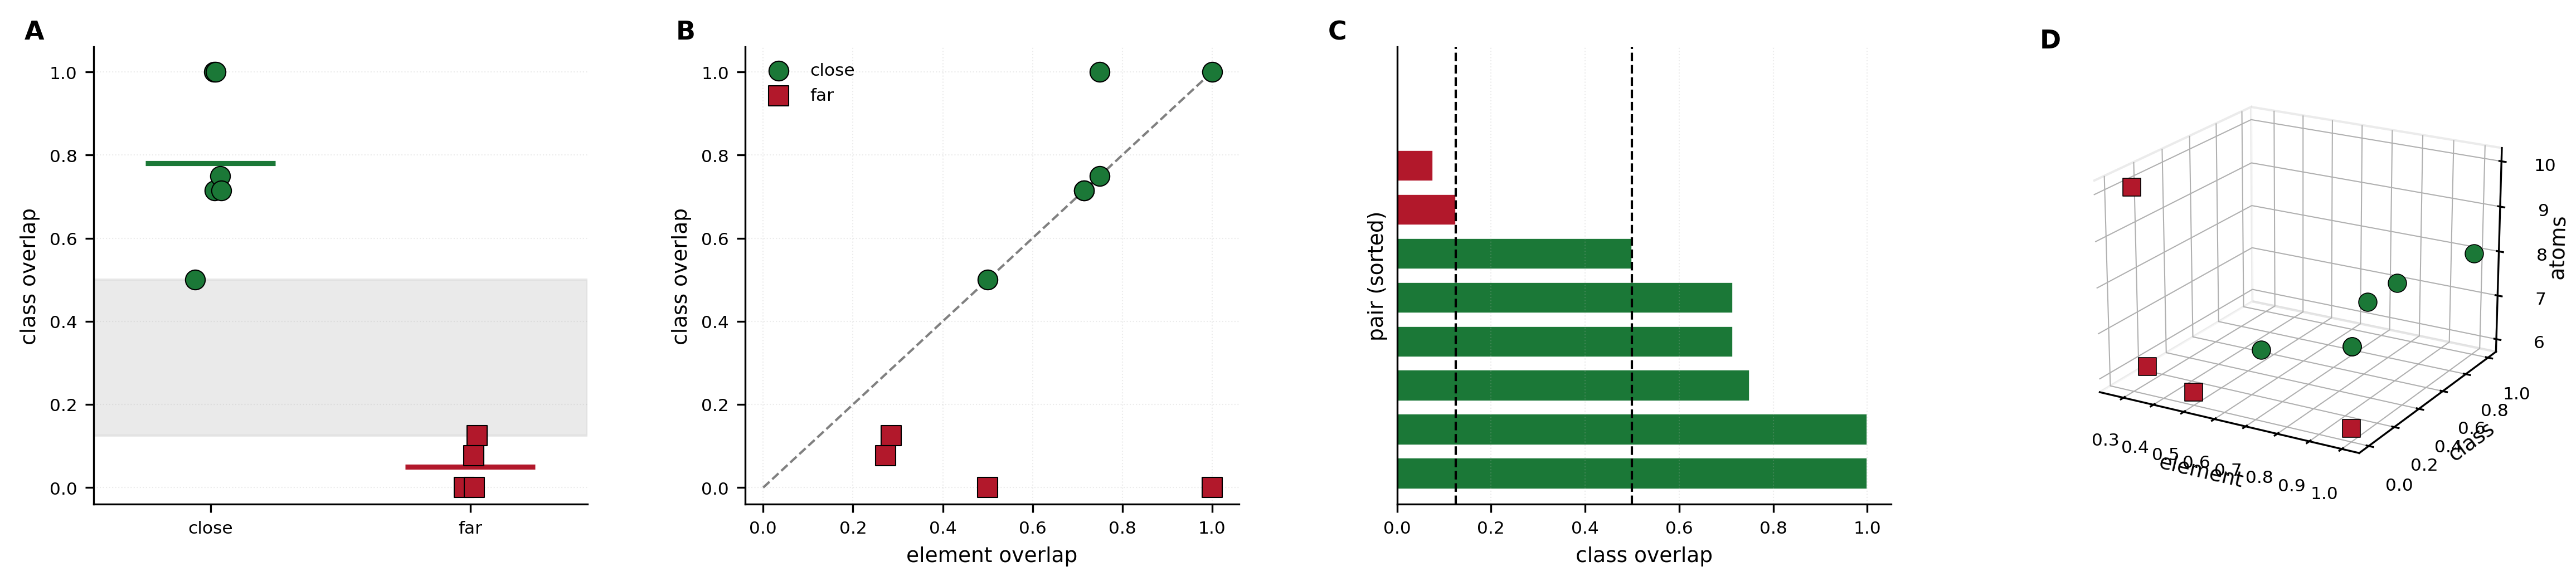
\includegraphics[width=\textwidth]{panel_02_separation.png}
\caption{\textbf{Separation of the annotated groups at the working radius.}
(\textbf{A})~Class overlap for the two groups with horizontal bars at the group
means; the shaded band is the gap between the highest \textsf{far} value
($0.125$) and the lowest \textsf{close} value ($0.500$), which no pair occupies.
(\textbf{B})~Class overlap against element overlap per pair with the identity
line: the two \textsf{far} points on the floor at element overlap $0.5$ and $1.0$
are pairs an element-keyed comparison cannot distinguish and the cut class
separates completely. (\textbf{C})~All ten pairs sorted by class overlap, with
the two dashed lines marking the boundaries of the empty band.
(\textbf{D})~Element overlap, class overlap and structure size in three
dimensions, showing that the separation is not an artefact of the pairs having
different sizes.}
\label{fig:separation}
\end{figure*}

\subsection{Separation of bioisosteric from unrelated pairs}

\begin{table}[htbp]
\centering\small
\caption{Class overlap at radius $0$ on the annotated pairs. The
\textsf{close}/\textsf{far} annotation was fixed before measurement.}
\label{tab:pairs}
\begin{tabular}{@{}llrr@{}}
\toprule
Pair & Annotation & Class overlap & Element overlap\\
\midrule
phenol / thiophenol & close & $1.000$ & $0.750$\\
catechol / resorcinol & close & $1.000$ & $1.000$\\
phenol / aniline & close & $0.750$ & $0.750$\\
benzene / pyridine & close & $0.714$ & $0.714$\\
pyridine / pyrimidine & close & $0.714$ & $0.714$\\
benzene / pyrazine & close & $0.500$ & $0.500$\\
\midrule
ethanol / benzene & far & $0.125$ & $0.286$\\
acetone / naphthalene & far & $0.077$ & $0.273$\\
benzene / cyclohexane & far & $0.000$ & $1.000$\\
propane / pyridine & far & $0.000$ & $0.500$\\
\midrule
ethanol / benzene        & far   & $0.000$ & $0.125$\\
propane / pyridine       & far   & $0.000$ & $0.125$\\
acetone / naphthalene    & far   & $0.000$ & $0.077$\\
benzene / cyclohexane    & far   & $0.125$ & $1.000$\\
\midrule
mean close & & $0.780$ & \\
mean far   & & $0.050$ & \\
\bottomrule
\end{tabular}
\end{table}

The ranges are disjoint: the lowest \textsf{close} overlap is $0.500$ and
the highest \textsf{far} overlap is $0.125$, a margin of $0.375$
(\Cref{tab:pairs}).

The benzene/cyclohexane row is the most informative in the table. Element
overlap is $1.000$---both are rings of six carbons---so an element-keyed
comparison regards them as compositionally identical. Class overlap is
$0.000$: an aromatic ring carbon and a saturated ring carbon receive
different cut keys, and the two structures share no class at all. This is
a case where the invariant discriminates exactly where element identity
cannot, and it is the reason the 	extsf{far} group's element overlaps in
\Cref{tab:pairs} are not uniformly small while its class overlaps are.


\begin{figure*}[!htbp]
\centering
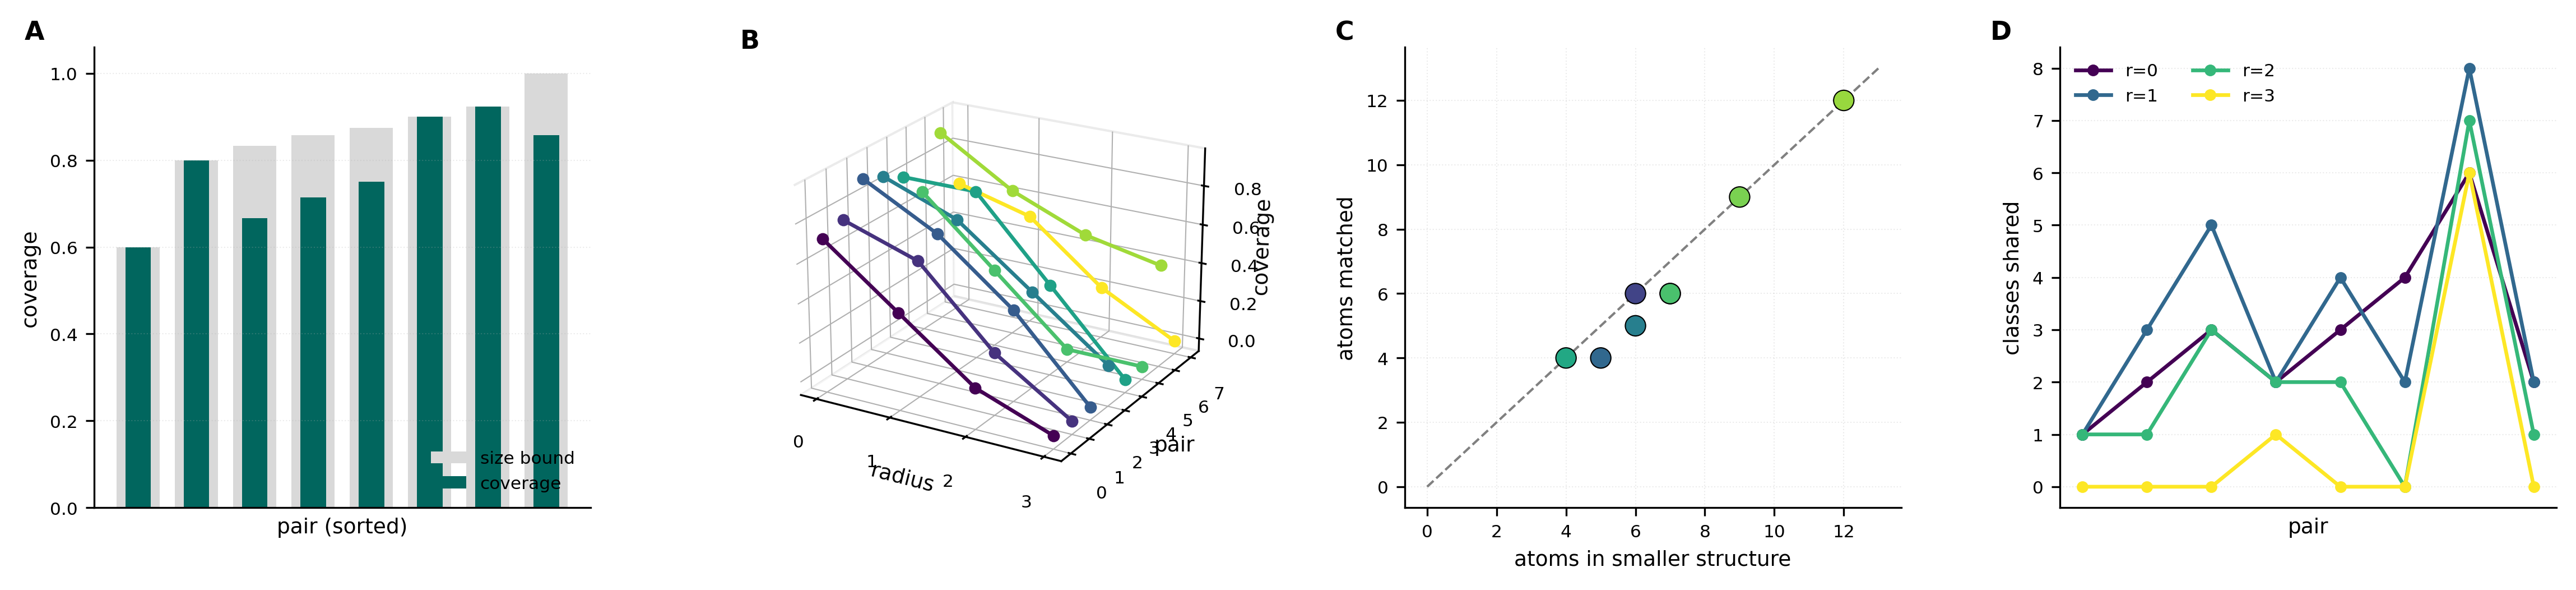
\includegraphics[width=\textwidth]{panel_03_correspondence.png}
\caption{\textbf{Correspondence on matched pairs and its decay with radius.}
(\textbf{A})~Coverage (teal) against the size bound $\min(n_1,n_2)/\max(n_1,n_2)$
(grey) per pair, sorted; three of the eight pairs reach their ceiling, so raw
coverage understates the match quality for pairs of unequal size.
(\textbf{B})~Coverage against radius for each matched pair in three dimensions;
every pair loses coverage monotonically as the labelling discriminates more.
(\textbf{C})~Atoms matched against the atom count of the smaller structure, with
the identity line and colour by coverage; points on the line are pairs in which
every atom of the smaller structure found a correspondent. (\textbf{D})~Classes
shared between the two structures of each pair at each radius, showing the same
erosion from a different quantity.}
\label{fig:corr}
\end{figure*}

\subsection{Correspondence on matched pairs}

\begin{table}[htbp]
\centering\small
\caption{Correspondence coverage at radius $0$ on pairs differing at one
position.}
\label{tab:matched}
\begin{tabular}{@{}lrrrr@{}}
\toprule
Pair & $n_1$ & $n_2$ & matched & coverage\\
\midrule
phenylalanine / tyrosine & $12$ & $13$ & $12$ & $0.923$\\
benzoic / salicylic & $9$ & $10$ & $9$ & $0.900$\\
aniline / phenol & $7$ & $7$ & $6$ & $0.857$\\
propanol / butanol & $4$ & $5$ & $4$ & $0.800$\\
phenol / cresol & $7$ & $8$ & $6$ & $0.750$\\
benzene / toluene & $6$ & $7$ & $5$ & $0.714$\\
glycine / alanine & $5$ & $6$ & $4$ & $0.667$\\
pyridine / quinoline & $6$ & $10$ & $6$ & $0.600$\\
\midrule
\textbf{mean} & & & & $\mathbf{0.776}$\\
\bottomrule
\end{tabular}
\end{table}

Coverage is bounded above by $\min(n_1,n_2)/\max(n_1,n_2)$, so the
pyridine/quinoline row---six atoms against ten---cannot exceed $0.600$,
and it attains that bound exactly: every atom of the smaller structure is
matched. The same holds for benzoic/salicylic at $0.900$. Reading
\Cref{tab:matched} as a measure of matching quality therefore requires
normalising by the size bound, which we have not done; raw coverage is
reported, and three of the eight rows are at their ceiling.

\subsection{The weakest result: cross-element pairings}

The claim that tolerance is doing work rests on the correspondence
admitting pairings an element-keyed matcher cannot make. We counted them.

\begin{table}[htbp]
\centering\small
\caption{Pairings admitted at radius $0$ on the \textsf{close} pairs,
split by whether the two atoms are the same element.}
\label{tab:cross}
\begin{tabular}{@{}lrrr@{}}
\toprule
Pair & total pairings & same-element & cross-element\\
\midrule
catechol / resorcinol & $8$ & $6$ & $2$\\
phenol / aniline & $6$ & $5$ & $1$\\
phenol / thiophenol & $7$ & $6$ & $1$\\
benzene / pyridine & $5$ & $5$ & $0$\\
benzene / pyrazine & $4$ & $4$ & $0$\\
pyridine / pyrimidine & $5$ & $5$ & $0$\\
\midrule
\textbf{total} & $\mathbf{35}$ & $\mathbf{31}$ & $\mathbf{4}$\\
\bottomrule
\end{tabular}
\end{table}

Four cross-element pairings across six pairs, in three of the six
(\Cref{tab:cross}). Mean coverage is $0.865$ with cross-element pairings
admitted and $0.776$ without.

This is a real effect and a small one, and we report it as the paper's
least convincing measurement. The gain concentrates in pairs where the
substituted atom is peripheral (the O/N of phenol/aniline, the two
hydroxyls of catechol/resorcinol) and vanishes where the heteroatom sits
inside a ring, because there the substitution changes the ring's cut
structure enough that the corresponding atoms no longer share a key. A
larger corpus would establish whether that pattern holds; six pairs
cannot.


\begin{figure*}[!htbp]
\centering

\includegraphics[width=\textwidth]{panel_04_control.png}
\caption{\textbf{The rewiring control and the cross-element gain.}
(\textbf{A})~Separation margin for the true structures ($+0.375$) and after
rewiring the second structure of each pair at random while holding atom
composition and edge count fixed ($-0.069$): the separation does not survive.
(\textbf{B})~Group means before and after rewiring; the \textsf{close} mean
collapses from $0.780$ to near the \textsf{far} value, while the \textsf{far}
mean barely moves. (\textbf{C})~Margin over radius under both conditions in three
dimensions: the true margin exists only at radius $0$ and the rewired margin is
negative everywhere. (\textbf{D})~Pairings admitted per \textsf{close} pair split
into same-element (blue) and cross-element (orange); the cross-element pairings,
which an element-keyed matcher cannot make, total $4$ across the six pairs and
occur in three of them.}
\label{fig:rewire}
\end{figure*}

\subsection{Negative control}

\begin{table}[htbp]
\centering\small
\caption{Rewiring control: the second structure of each pair is rewired at
random, holding atom composition and edge count fixed, and rescored
($20$ seeds per pair).}
\label{tab:control}
\begin{tabular}{@{}lr@{}}
\toprule
Quantity & Margin\\
\midrule
True structures & $+0.375$\\
Rewired structures & $-0.069$\\
\bottomrule
\end{tabular}
\end{table}

Rewiring collapses the separation and reverses its sign
(\Cref{tab:control}), so the overlap at radius $0$ is measuring structure
and not composition.

\subsection{Two experiment-design errors}
\label{sec:errors}

Two components of this suite were wrong when first written, and both are
recorded because each would have supported a conclusion the data do not.

\paragraph{A control that could not fail.} The first negative control
permuted class labels \emph{within} each structure, on the reasoning that
this destroys the structural assignment. It does not: a multiset is
invariant under relabelling of its elements, so the shuffled score equalled
the true score exactly and the control reported a margin identical to the
real one. A control that cannot fail certifies nothing. The replacement
rewires the graph, holding composition fixed, and does collapse the margin
(\Cref{tab:control}).

\paragraph{A baseline that was not a baseline.} The first element baseline
compared multisets of $(\text{element},\text{degree})$ pairs. On this
corpus that is very nearly the cut key itself, so the two scored almost
identically and the comparison appeared to show the method adding nothing.
The error was in the baseline: an element-keyed matcher's actual
constraint is exact element identity, and the place it binds is the
correspondence, not the multiset. \Cref{tab:cross} is the replacement,
and it gives a smaller effect than the flawed comparison would have
suggested in the other direction.

\subsection{What the suite does not establish}

The corpus is ten annotated pairs, eight matched pairs and thirty
structures, all hand-assembled. The \textsf{close}/\textsf{far}
annotations encode our reading of the medicinal-chemistry literature and
are not derived from activity data. Nothing here measures retrieval
performance, enrichment, or agreement with any experimental endpoint. With
six \textsf{close} pairs, no statistical statement about the cross-element
effect is warranted, and none is made.

% =====================================================================

\begin{figure*}[!htbp]
\centering
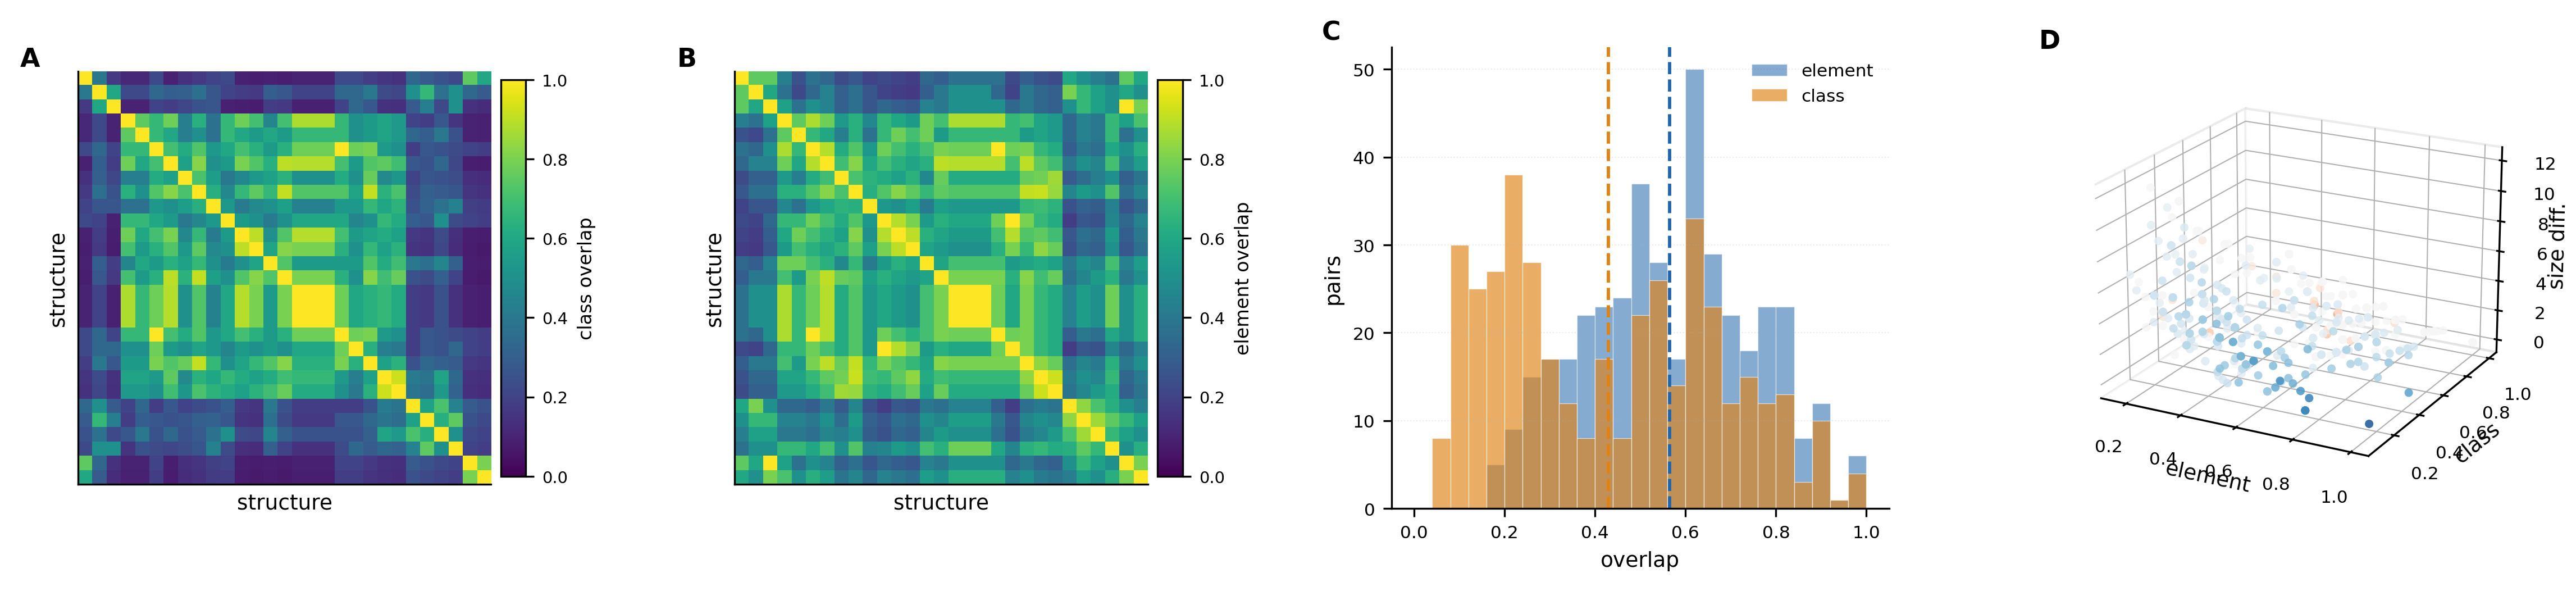
\includegraphics[width=\textwidth]{panel_05_matrix.png}
\caption{\textbf{Class and element overlap over the drug-like set.}
(\textbf{A})~Class-overlap matrix for all $\binom{30}{2}$ pairs of the drug-like
corpus at radius $0$, structures in corpus order. (\textbf{B})~Element-overlap
matrix for the same pairs on the same scale; the block structure differs
visibly, so the two quantities are not proxies for one another.
(\textbf{C})~Distributions of the two overlaps over the $406$ pairs with their
means marked: class overlap is shifted toward lower values, because agreeing on
composition is easier than agreeing on structural role. (\textbf{D})~Element
overlap, class overlap and absolute size difference in three dimensions,
coloured by class minus element overlap; points far from the diagonal plane are
pairs on which the two criteria most disagree.}
\label{fig:matrix}
\end{figure*}

\section{Relation to existing methods}
\label{sec:related}
% =====================================================================

\paragraph{Maximum common substructure.} MCS finds the largest common
connected or disconnected subgraph and is $\mathsf{NP}$-hard
\citep{garey1979,raymond2002,ehrlich2011}, normally attacked as clique
detection on a modular product \citep{barrow1976,bron1973} or by
specialised search \citep{cao2008,dalke2013}. The present construction
does not compute an MCS and is not an approximation to one: it returns a
vertex correspondence with no connectivity guarantee
(\Cref{sec:limits}). The tractability follows from solving a weaker
problem, not from a better algorithm for this one.

\paragraph{Substructure search.} Subgraph isomorphism
\citep{ullmann1976,cordella2004,ehrlich2012} requires element identity by
definition of the problem. Our matcher answers a different question and
should not be substituted for it.

\paragraph{Bioisostere databases.} Systematic replacement catalogues
\citep{wirth2013} are derived from observed medicinal-chemistry practice
and are therefore limited to substitutions someone has made. A computed
invariant proposes correspondences for pairs nobody has catalogued; it
also has no evidence behind any particular one, which is the reverse
trade.

\paragraph{Fingerprint similarity.} Circular fingerprints
\citep{rogers2010} and the similarity measures built on them
\citep{willett1998,maggiora2014} give a number per pair. The present
construction gives a correspondence, from which a number can be derived
(\Cref{def:overlap}) but which also says which atoms play which roles.
Whether the number is better than a fingerprint's is not measured here.

\paragraph{Colour refinement.} The iteration \eqref{eq:refine} is a colour
refinement \citep{weisfeiler1968,arvind2015}. We use it in the opposite
direction from its usual purpose: rather than refining as far as possible
to distinguish structures, we refine as little as possible in order to
identify them.

% =====================================================================
\section{Limitations}
\label{sec:limits}
% =====================================================================

\begin{enumerate}[label=\textbf{L\arabic*.},leftmargin=2.8em,itemsep=4pt]

\item \textbf{The correspondence is not connected.} \Cref{def:corr}
matches atoms by label and imposes no requirement that matched atoms form
a connected subgraph or that bonds are preserved. It is therefore not a
common substructure in any sense, and reporting its size as an MCS size
would be wrong.

\item \textbf{Within-class assignment is arbitrary.} When a label class
has several members on both sides, \Cref{def:corr} zips them in a fixed
order. Which member pairs with which is a convention, and a different
convention gives a different correspondence of the same size. Only the
size and the class structure are invariant (\Cref{thm:invariance}); the
individual pairings are not.

\item \textbf{The cross-element gain is small.} Four pairings across six
molecule pairs (\Cref{tab:cross}). This is the measurement most in need of
a larger corpus, and it is the one the paper's motivation leans on hardest.

\item \textbf{Corpus scale and construction.} Ten annotated pairs, eight
matched pairs, thirty structures, all chosen by us. The
\textsf{close}/\textsf{far} labels are our reading of the literature, not
measurements. A corpus we assembled to exhibit a property is weak evidence
that anything else has it \citep{ioannidis2005}.

\item \textbf{No endpoint validation.} Nothing here is tested against
binding data, activity cliffs \citep{stumpfe2012}, or any retrieval
benchmark.

\item \textbf{The weighting is an input.} \Cref{def:graph} requires only
$\wt>0$; every theorem holds for any positive weighting and none
determines one. The measurements use a weighting derived from valence
arithmetic. Different weights give different keys and could give a
different sweep.

\item \textbf{Coverage is not normalised.} \Cref{tab:matched} reports raw
coverage, which is bounded by the size ratio of the two structures. Pairs
of unequal size are penalised by that bound rather than by any matching
failure.

\item \textbf{Colour-refinement limits are inherited.} At any radius the
labelling is a colour refinement and cannot distinguish structures that
refinement cannot distinguish \citep{arvind2015}. At radius $0$ this is
severe by design---that is the tolerance---but it means the matcher will
identify atoms that are genuinely different whenever their cut keys
coincide.
\end{enumerate}

% =====================================================================
\section{Conclusion}
\label{sec:conclusion}
% =====================================================================

We have defined a structural correspondence keyed on a minimum-cut
invariant rather than on element identity, shown that it is symmetric,
invariant and computable without search
(\Cref{thm:symmetry,thm:invariance,prop:cost}), and established that its
tolerance is a resolution parameter: refinement radius trades tolerance
for discrimination monotonically (\Cref{lem:radius-order},
\Cref{prop:overlap-monotone}).

The measurement that most changed our understanding was the radius sweep.
We predicted the coarsest radius would separate bioisosteric from
unrelated pairs best, and it does---margin $+0.375$ at radius $0$ against
exactly $0$ at radii $1$, $2$ and $3$. The instinct to make a matcher more
discriminating is wrong for this task, and the sweep is what shows it.

At the working radius, class overlap separates the annotated groups with
disjoint ranges ($0.780$ against $0.050$; minimum close $0.500$, maximum
far $0.125$), a rewiring control collapses that margin to $-0.069$, and
correspondence coverage on one-position matched pairs averages $0.776$.
The benzene/cyclohexane pair is the clearest single illustration:
identical under element composition, well separated under cut class.

Two design errors are recorded in \Cref{sec:errors}---a control that could
not fail and a baseline that was not one---because each would have
supported a conclusion the corrected measurement does not. And the
cross-element result, which is the effect the whole motivation rests on,
is four pairings across six pairs: real, small, and in need of a corpus
larger than the one we assembled.

\section*{Reproducibility}

The experiment source records each expectation before its measured value
and writes every reported quantity to a JSON results file. The corpus,
including the \textsf{close}/\textsf{far} annotations, is in the source
with the reasoning for each entry. All minimum cuts are computed exactly;
the only stochastic component is the rewiring control, which seeds
explicitly and reports the seed range.

\bibliographystyle{plainnat}
\bibliography{references}

\end{document}
